\chapter{物质的导电性}\label{chp:conductivity}
我们知道,容易导电的物质叫做导体,不容易导电的物质叫做绝缘体。
金属是导体,能够导电,这是大家都熟悉的。
除了金属之外,有的液体和气体也能够导电,但是它们跟金属导电情况并不完全相同。
还有一类物质,介于导体和绝缘体之间,叫做半导体,又有自己的导电特点。
这一章,我们将根据物质的微观结构来讨论各种物质的导电性。

\section{金属的导电性}
在常温下,金属一般都是晶体。
金属晶体的空间点阵是由金属原子释放出价电子后形成的金属离子组成的。
释放出的价电子可以在整个金属晶体里自由运动,叫做\Concept{自由电子}。
金属导体就是靠自由电子来导电的,这种导电现象叫做\Concept{电子导电}。

通常情况下,金属中的自由电子不断地做无规则的热运动,它们朝任何方向运动的机会都一样。
从宏观上看,没有电荷(自由电子)的定向移动,因而也没有电流(参看\cref{fig:7-1})。
如果导体的两端有电势差,在导体内部就建立了电场,导体中的自由电子就要受到电场力的作用。
这样,自由电子在导体中除了做无规则的热运动外,还要在电场力的作用下定向移动,形成电流。

金属导体中的电流强度跟自由电子的定向移动速率有关系,它们之间的关系可以用下述的方法简单计算出来。
\begin{figure}
  \includegraphics{8-1.pdf}	
  \caption{}\label{fig:8-1}
\end{figure}

如\cref{fig:8-1} 所示,设金属导体的横截面积为 $S$,自由电子密度(单位体积内的自由电子数)为 $n$,自由电子平均定向移动速率为 $v$,那么时间 $t$ 内通过某一横截面的自由电子数为 $nSvt$。
如果电子的电量为 $e$,那么时间 $t$ 内通过横截面的电量 $q=neSvt$。
根据电流强度的公式 $I=q/t$,就可以得到电流强度和自由电子平均定向移动速率的关系式:
\[I=neSv.\]

设横截面积为 \qty{1.0}{mm^2} 的铜导线中通过 \qty{1.0}{A} 的电流,铜的自由电子密度为 \qty{8.5e28}{m^3},电子的电量为 \qty{1.6e-19}{C},由上式可以算出这时自由电子平均定向移动速率是 \qty{7.4e-5}{m/s}。
而常温下金属中自由电子热运动平均速率约为 \qty{e5}{m/s}。可见,在金属导电的时候,自由电子只不过在速率巨大的无规则热运动上附加了一个速率很小的定向移动就是了。

既然自由电子定向移动的速率很小,为什么我们合上开关,电流会立即传到远处,使那里的用电器工作呢?
原来,我们觉察到的“电的传播速率”不是自由电子的定向移动速率,而是电场的传播速率,电场的传播速率是很大的,等于光速(\qty{3e8}{m/s})。
在电路未接通前,电路里没有电场,自由电子没有定向移动。
电路一且接通,电路里便以 \qty{3e8}{m/s} 的速率在各处极迅速地建立起电场,在这个电场作用下,电路里各处的自由电子几乎同时立即开始做定向移动,整个电路中几乎同时形成了电流。

金属导体中的电流是自由电子的定向移动形成的,从这种电子论的观点可以对欧姆定律作出微观解释。
\begin{figure}
  \includegraphics{8-2.pdf}
  \caption{}\label{fig:8-2}
\end{figure}

如\cref{fig:8-2} 所示,设有一段金属导体,横截面积为 $S$,长度为 $l$。
如果导体的两端有电压 $U$,导体中的电场强度就是 $E=U/l$。
这时,作用在自由电子上的电场力 $F=eE$。
自由电子正是在这个力的作用下做定向移动的。
设电子的质量为 $m$,根据牛顿第二定律可以求出自由电子定向移动的加速度
\[a=\frac{F}{m}=\frac{eE}{m}=\frac{e}{ml}U.\]

运动的自由电子要频繁地跟金属正离子碰撞,结果使自由电子的定向移动很快受到破坏,限制了定向移动速率的继续增加。
自由电子在碰撞后向各个方向弹射的机会相等,因而失去了碰撞前具有的定向移动的特性,又要从新开始做初速为零的定向加速运动。

自由电子相继两次碰撞的时间间隔有长有短,设平均时间为 $\tau$,那么,自由电子在下次碰撞前的定向移动速率 $v_{\tau}=a\tau$,在时间 $\tau$ 内的平均定向移动速率
\[v=\frac{1}{2}v_{\tau}=\frac{1}{2}a\tau.\]
这样,对大量电子来说,可以认为每个电子都以这个平均定向移动速率做定向移动。
上面已经得出
\[a=\frac{e}{ml}U,\]
因此,自由电子平均定向移动速率
\[v=\frac{e\tau}{2ml}U.\]
把此式代入前面推出的公式 $I=neSv$ 中得
\[I=\frac{e^2 nS\tau}{2ml}U.\]

{\linespread{1.65}\selectfont 对于一定的金属材料,在一定的温度下,$\tau$ 是个确定的数值(\qtyrange{e-14}{e-12}{s})。这就是说,对于一段金属导体,$\dfrac{e^2 nS\tau}{2ml}$ 是一个常量。因此,我们得到,导体中的电流强度 $I$ 跟这段导体两端的电压 $U$ 成正比,这正是欧姆定律告诉我们的。\par}

这种以经典物理为基础的电子论(经典电子论)虽然能对金属导电规律作出解释,但它只能给出金属导体的电子导电的概况,而不能获得满意的定量的结果。
例如,对于金属导体的电阻跟温度的关系,从电子论得到的是电阻跟温度的平方根成正比,而实验结果却是电阻跟温度成正比。
这说明经典电子论本身存在着缺陷。
近代物理指出,只有用量子理论来研究金属导电,才能得到与实验相符合的结果。

\begin{Practice}
\begin{question}
  \item 在金属导体中,自由电子的热透动速率和定向移动逮率之间有什么区别?这两种速率哪个大?
  \item 电路接通后,为什么整个电路中几乎同时形成电流?
  \item 利用公式 $I=\dfrac{e^2 nS\tau}{2ml}U$,求出这段导体的电阻 $R$ 和制成这段导体的材料的电阻率 $\rho$。
\end{question}
\end{Practice}

\section{液体的导电性}
我们在化学中学过,酸、碱、盐是电解质,它们的水溶液或者它们熔解成的液体能够导电,这就是液体导电。
液态金属也能够导电,也属于液体导电。
液态金属的导电情况跟固态金属相同,都是电子导电,这里不再讨论,这一节,我们讨论电解质导电。

电解质在水溶液中或者熔解成液体时都要发生电离,它们的分子电离成正离子和负离子。
这些离子不断地做无规则的热运动,没有电场存在时,从宏观上看没有电荷(离子)的定向移动,不显示出电流。

\medskip\noindent
\begin{minipage}{0.5\linewidth}\parindent2em
在电解质的液体里插入两个电极,把它们分别接在电源的正负极上,跟电源正极相连的叫阳极,跟电源负极相连的叫阴极。
于是液体中出现电场,电解质的正负离子除了做热运动外,还要在电场力的作用下散定向移动,正离子向阴极移动,负离子向阳极移动。
电解质就是靠正负离子的定向移动形成电流的。
这种导电现象叫做\Concept{离子导电}。
显然,这跟金属中的电子导电是不同的。
\end{minipage}\hfill
\begin{minipage}{0.45\linewidth}\centering
  \begin{figurehere}
    \includegraphics{8-3.pdf}
    \caption{}\label{fig:8-3}
  \end{figurehere}
\end{minipage}

\medskip
在电解质导电过程中,同时发生电解现象。
电解时,正离子在阴极板上得到电子发生还原反应,负离子在阳极板上失去电子发生氧化反应,电解质的导电过程要发生化学变化,这也是跟金属导电不同的。
金属导电时,金属本身并不发生化学变化。
例如,在氯化铜溶液中氯化铜分子电离成铜离子 \ce{Cu^2+} 和氯离子 \ce{Cl-}。
导电时,带正电的铜离子向阴极移动,带负电的氯离子向阳极移动(\cref{fig:8-3})。
在阳极,氯离子失去电子而氧化成中性氯原子,两个氯原子又结合成氯分子,从阳极放出。在阴极,铜离子获得电子而还原成中性铜原子,就覆盖在阴极上。

电解在工业上有着广泛的应用,如电镀、电冶、电解精炼等。
这些都已在化学课学习过,这里就不再重复了。
利用电解还可以使金属表面氧化。
例如,把铝板放在硼酸或硼砂的水溶液中作为阳极,利用电解现象,可以在铝的表面得到非常薄的氧化膜,这个氧化膜有良好的绝缘性。
因此,把铝作阳极,把电解液作阴极,可以做成电容量很大的电容器。
这就是电解电容器。
由于电解电容器是利用电解产生的绝缘膜作电介质的,因此把它连在电路中时,它的正负极不能接反,并且不能接在交流电路中。

\section{法拉第电解定律}
电解质导电时,要发生化学变化,有物质在极板处析出。
那么,析出的物质的质量跟通电的电流强度和时间有什么关系呢?

这个关系可以用实验来确定。
给某种电解质溶液通电,先使各次的通电时间相同,而电流强度不相同,再使各次通电的电流强度相同,而时间互不相同,每次都精密地测出极板(阳极或阴极)处析出的物质的质量。
实验结果表明:在通电时间相同的情况下,析出物质的质量跟电流强度成正比;在电流强度相同的请况下,析出物质的质量跟通电时间成正比。
例如,氯化铜溶液电解时,从阳极放出的氯气的质量或在阴极上得到的铜的质量都跟通电的时间和电流强度成正比。

\emph{电解质导电时,在极板处析出的物质的质量 $m$ 跟通电时间 $t$ 和电流强度 $I$ 成正比,或者说跟通过电解液的电量 $q$ 成正比}。
这就是\Concept{法拉第电解第一定律},写成公式就是
\begin{equation}
  \label{eq:Faraday_law_1}
    m=kIt=kq.
\end{equation}
式中的 $k$ 是比例恒量,叫做\Concept{电化当量}。
从实验知道,电化当量的数值随着被析出的物质种类而不同。
某种物质的电化当量在数值上等于通过 \qty{1}{C} 电量时析出的这种物质的质量。
电化当量 $k$ 的单位是千克/库(\unit{kg/C})。

\begin{table}
  \caption{几种物质的电化当量和化学当量}\label{tab:8-1}
\begin{tblr}{colspec={X[c]X[2,r]X[2,r]},hline{2}=0.8pt,row{1}={m,c}}
物质        &  电化当量 $k$(\qty{e-8}{kg/C})  &  化学当量 $M/n$(\qty{e-8}{kg/mol})\\
\ce{H^+}    &  0.01044    &    1.0079   \\
\ce{Al^3+}  &  0.00317    &    8.9938   \\
\ce{Fe^3+}  &  0.1930     &   18.6157   \\
\ce{Cu^2+}  &  0.3294     &   31.772    \\
\ce{Ag+}    &  1.118      &  107.868    \\
\ce{O^2-}   &  0.0829     &    7.9997   \\
\ce{Cl-}    &  0.3672     &   35.453    \\
\ce{OH-}    &  0.1762     &   17.007    \\
\ce{SO4^2-} &  0.4975     &   48.029    \\
\ce{NO_3^-} &  0.642      &   62.005    \\
\end{tblr}
\end{table}

电化当量 $k$ 可以从实验得出,通过电解质的电流强度 $I$、通电时间 $t$ 和析出物质的质量 $m$ 都可以由实验测定,根据法拉第电解第一定律就可以求出 $k=m/(It)$。\cref{tab:8-1} 的第二列给出了几种物质的电化当量。

知道了物质的电化当量,就可以由通电时间和电流强度求出析出的物质的质量。

物质的电化当量又跟物质的什么性质有关呢?
法拉第在大量实验事实的基础上指出:\emph{物质的电化当量跟它的化学当量成正比},这就是\Concept{法拉第电解第二定律}。

某物质的化学当量是该物质的摩尔质量 $M$ 跟它的化合价 $n$ 的比值,化学当量的单位是千克/摩(\unit{kg/mol})。
例如,铜的摩尔质量是 \qty{0.063546}{kg/mol},二价铜的化合价 $n=2$,所以它的化学当量 $M/n$ 等于摩尔质量的一半,即 \qty{0.031772}{kg/mol}。
\cref{tab:8-1} 第三列给出了几种物质的化学当量。

通常,电化当量 $k$ 跟化学当量 $M/n$ 之间的比例常数用 $1/F$ 来表示,于是法拉第电解定律可用公式表示为
\begin{equation}
  \label{eq:Faraday_law_2}
  k=\frac{M}{Fn}.
\end{equation}

式中的 $F$ 叫做\Concept{法拉第恒量},对于任何物质都是相同的,实验测量结果表明,$F=\qty{9.65e4}{C/mol}$。
同学们根据\cref{tab:8-1} 中的两列数据,算一算各种物质的电化当量 $k$ 跟化学当量 $M/n$ 的比值,就会得到它们的比值是相同的。

法拉第恒量的意义是什么呢?
把电解第二定律的公式 \eqref{eq:Faraday_law_2} 代入电解第一定律的\cref{eq:Faraday_law_1}中,得到
\begin{equation}
  m=\frac{M}{Fn}q.
\end{equation}

上式中如果 $m$ 的数值等于 $M/n$ 的数值,那么 $F$ 的数值等于 $q$。
可见,\emph{法拉第恒量在数值上等于析出数值等于化学当量的物质时,需要通过电解质的电量}。
例如一价银的化学当量是 \qty{0.107868}{kg/mol},析出 \qty{0.107868}{kg} 的银,需要 \qty{9.65e4}{C} 的电量。
二价铜的化学当量是 \qty{0.031772}{kg/mol},析出 \qty{0.031772}{kg} 的铜,也需要 \qty{9.65e4}{C} 的电量。

\section{电子电量的确定}
法拉第电解定律是实验定律。
法拉第发现电解定律时,人们还不清楚物质的分子、原子结构,也不知道存在着电子。
然而,法拉第电解定律的发现,给予人们有益的启示,为人们认识基本电荷起了重要作用。

我们知道,电解质导电是离子导电,而每种离子都带有一定的电荷。
因此,在电极处析出一定质量的某物质,就表明有一定数量的这种物质的离子到达电极。
到达电极的离子数越多,通过电解质的电量就越多,析出的物质也就越多。
这就是电解第一定律所表达的内容。

下面我们进一步指出,根据电解第二定律所确定的法拉第恒量,我们可以算出离子所带的电量,而一价离子所带的电量就等于电子的电量,即基本电荷。

我们知,在数值等于化学当量 $M/n$ 的物质中,含有的离子数是 $N/n$,其中 $N$ 是阿伏伽德罗常数,等于 \qty{6.02e23}{mol^{-1}}。
有 $N/n$ 个离子到达电极,通过电解质的电量的数值等于 $F$,为 \num{9.65e4}。
因此,$n$ 价离子所带的电量 $q_n$ 是:
\[q_n=\frac{F}{N/n}=n\frac{F}{N}.\]

对于一价离子,$n=1$,$q_n$ 就等于电子的电量,即
\[e=\frac{F}{N}.\]

可见,知道了法拉第恒量 $F$ 和阿伏伽德罗常数 $N$,就可以求出电子的电量 
\[e=\frac{F}{N}=\frac{\num{9.65e4}}{\num{6.02e23}}=\qty{1.60e-19}{C}.\]
这个结果跟用其他方法(例如\cref{chp:electric_field}讲的密立根实验)求得的电子电量的数值是一致的。

实际上,公式 $e=F/N$ 把法拉第恒量、基本电荷、阿伏伽德罗常数这三者联系起来了。
测出法拉第恒量和阿伏伽德罗常数,可以求出基本电荷;测出法拉第恒量和基本电荷,也可以求出阿伏伽德罗常数。

\begin{Reading}{$e$ 和 $N$ 的测定}
电子电量 $e$ 和阿伏伽德罗常数 $N$ 都是物理学的基本常数。
从公式 $e=F/N$ 可以看出,在 $e$ 和 $N$ 这两个常数的测定中,如果有一个常数有了新的测定数值,另一个的数值就要随着变化,二者的数值测定明显地有着互相推动的作用。

阿伏伽德罗常数最早是洛喜密脱于 1865 年左右根据分子运动论所确定的关系来测定的,二十世纪初又有人利用研究布朗运动所得到的关系以及利用其他方法来测定它的数值。
但是,这些方法本身都有缺点,所得的结果都不很准确。

直到 1917 年,美国物理学家密立根用油滴法测出了电子电量,并利用已知的法拉第常数,由公式 $e=F/N$ 求出阿伏伽德罗常数,这才有了在当时看来准确度较高的结果。

1928 年,瑞典物理学家贝克林利用 X 射线的方法测得了阿伏伽德罗常数,反过来又求出电子电量,他得到的 $N$ 和 $e$ 的数值,跟密立根的结果相比有较大的差别。
尽管他的方法是合理的,然而当时普遍认为密立根的方法是无可怀疑的,因此两个结果到底哪一个较为准确,一时难于确定。

1932 年,日本的芝龟吉指出了密立根的结果出现误差的原因。
考虑到这个误差,1936 年贝克林和弗仑堡重新用油滴法测定电子电量,结果得到了跟 X 射线法十分接近的 $e$ 和 $N$ 的数值。
以后,又有人多次用两种方法测定 $e$ 和 $N$,得到了更加一致的结果。
这样,原来两种方法得到的 $e$ 和 $N$ 的数值的差别,在实验的基础上基本得到统一。$e$ 和 $N$ 的数值测定在物理学中具有重要意义。
随着科学技术的发展,人们在不断研究精确测定它们的方法。
\end{Reading}

\begin{Practice}
\begin{question}
  \item 通过硫酸铜溶液的电量是 \qty{2e4}{C},在阴极上能析出多少克铜?
  \item 如果要在表面积是 \qty{5}{cm^2} 的器件上,镀上一层 \qty{20}{\micro m} 厚的银层,需要通过多少库仑的电量?
  \item 有一个学生电解硫酸铜溶液来测定铜的电化当量。他在通电以前称一次阴极板,通电 \qty{25}{min} 以后再称一次,从而知道析出的铜的质量是 \qty{0.29}{g},还知道通过溶液的电流强度是 \qty{0.6}{A},从这些数据算出铜的电化当量是多少?
  \item 锌的摩尔质量是 \qty{0.06538}{kg/mol},它的化合价是 2,求锌的电化当量。
  \item 金的摩尔质量是 \qty{0.1972}{kg/mol},它的化合价是 3,要想使金电解池的阴极上析出 \qty{1}{g} 金,需要通过多少库的电量?
\end{question}
\end{Practice}


\section{气体的导电性}
在通常情况下,气体是不导电的。
例如,采用裸导线的输电线路,不会由于空气的存在而把电路连通,造成短路。
但是,在某些外界条件作用下,气体是可以导电的。
象\cref{fig:8-4} 所示的那样,取两个验电器,让一个带正电,另一个带负电,并使它们上端的金属球互相靠近。
如果空气是干燥的,验电器的带电状态将保持不变。
把酒精灯火焰置于两个金属球之间,可以看到两个验电器很快就不带电了,说明这时空气变成了导体,把两个验电器导通了。
\begin{figure}
  \includegraphics{8-4.pdf}
  \caption{}\label{fig:8-4}
\end{figure}

空气为什么会变成导体呢?

通常情况下,气体几乎完全是由中性的原子或分子组成的,因此它是不导电的。
而空气在火焰的作用下能够电离,部分中性分子变成带电的离子,结果气体变成导体。

不仅火焰能使气体电离,利用其他方法,例如用紫外线、X 射线或放射性元素发出的放射线照射,也能使气体电离。
能使气体电离的物质叫做\Concept{电离剂}。

气体电离后发生的导电现象叫做\Concept{气体放电}。

气体导电跟电解质导电相似,它们都是由于发生了电离而具有导电性的。
但是也有区别。
电解质电离时,分解成正离子和负离子;气体电离时,分解成正离子和电子。
在气体中也可以形成负离子,这是由于电子附在中性分子上的结果。
可见,气体中既有象金属中那样的电子导电,也有象电解质中那样的离子导电。

现在我们利用如\cref{fig:8-5} 的实验装置对气体放电现象作进一步的讨论。
放电管是装有两个电极的玻璃管,里面充有一定压强的气体,给两电极加上一定的电压,在电离剂的作用下,放电管里面的气体发生放电。
拿走电离剂,气体不再发生电离,放电现象也就停止。
但是,如果增大两电极间的电压,即使没有电离剂的作用,也能发生放电现象。

\begin{figure}
  \begin{minipage}[b]{0.48\linewidth}\centering
    \includegraphics{8-5.pdf}
    \caption{}\label{fig:8-5}
  \end{minipage}
  \nextfloat
  \begin{minipage}[b]{0.48\linewidth}
    \begin{minipage}{0.45\linewidth}\centering
      \includegraphics{8-6a.pdf}
      \subcaption{}\label{fig:8-6a}
    \end{minipage}
    \begin{minipage}{0.45\linewidth}\centering
      \includegraphics{8-6b.pdf}
      \subcaption{}\label{fig:8-6b}
    \end{minipage}
    \caption{}\label{fig:8-6}
  \end{minipage}
\end{figure}

在电离剂的作用下才能发生的气体放电现象叫做\Concept{被激放电}。
没有电离剂的作用而发生的气体放电现象叫做\Concept{自激放电}。

放电管里的气体,为什么在高电压下会发生自激放电呢?

通常,气体中总会有少量电子和离子。
电子在电场的作用下向阳极运动。
在前进的道路上,电子会碰到离子和中性原子。
在两次碰撞之间,由于电场力做功,电子的动能增加。
两电极间的电压越大,电场越强,电子的动能增加得就越大。
电压足够高,电场足够强,电子的动能增大到一定程度时,电子跟中性原子碰撞,就会从原子中打出电子,发生气体电离。
这种电子碰撞电离\footnote{实验结果表明,正离子在电场作用下跟中性原子碰撞时,很少使原子发生电离,因此,这里只讨论电子碰撞电离。}的过程,可以用\cref{fig:8-6} 来说明。
\cref{fig:8-6a} 表示碰撞前的情形,\cref{fig:8-6b} 表示碰撞后的情形。
碰撞后有两个电子,一个是跟原子相碰的电子,一个是从原子中打出来的电子,它们也要在电场中获得动能,并使被到的原子电离。

但是,单靠电子碰撞使气体电离并不能维持自激放电。
因为碰撞产生的所有电子都要向阳极方向运动,到达阳极后就停止了。
为了维持放电,必须使阴极能够源源不断地提供电子。
通常把阴极提供电子的过程叫做\Concept{电子发射}。

气体电离时产生的正离子,在向阴极运动时,也具有动能。
如果这个动能足够大,正离子跟阴极碰撞时,就会从阴极表面打出电子。
这些电子又会使气体发生电子碰撞电离,产生新的电子和正离子。
这就维持了气体电离,形成自激放电。

从上面的讨论可以得出,产生自激放电的条件是气体电离和阴极发射电子。

象上面讲的那样,正离子跟阴极碰撞使阴极发射电子,叫做正离子轰击发射。
然而相当多的情况是给阴极加热,使阴极在高温下发射电子,这叫做热电子发射。
如果你想对电子发射有进一步的了解,可以看一看下面的阅读材料:电子发射。

\begin{Reading}{电子发射}
维持自激放电,阴极要能够提供电子。
后面就要讲到的阴极射线管、示波管以及其他电子器件,它们的阴极都是能提供电子的源泉。
阴极的这种提供电子的过程叫做电子发射。

阴极为什么能够发射电子呢?

我们知道,金属制成的阴极里有许多自由电子。
这些自由电子在正离子间不停地做无规则的热运动。
当电子趋近金属表面时,它们所受的正离子向内的拉力将急剧增加,这种情况好象是金属表面对电子形成了一道壁垒。
通常条件下,自由电子的能量太小,几乎无法越出这个壁垒,只能局限在金属内部运动。
然而,可以设法增加自由电子的能量,或者设法减弱金属表面对自由电子逸出金属的阻力。
这样,自由电子就可以冲破金属表面壁垒的封锁,从金属里释放出来,这就是电子发射现象。

电子发射可以分为下列几种形式:
\begin{enumerate}
  \item 热电子发射。给金属加热,做热运动的自由电子的能量随着温度的升高而增大,其中一部分电子可以获得足够的能量,克服阻止它们逸出的阻力而逸出金属。
  \item 正离子轰击发射。气体电离产生的正离子,在电场力作用下高速运动而具有很大的动能,当它们跟阴极碰撞时,可以使一部分自由电子获得足够的能量,从阴极释放出来。
  \item 光电子发射。某些金属受到光的照射时,其中的一部分自由电子能够吸收足够的能量,而产生电子发射,这种电子发射也叫做光电效应。
  \item 场致电子发射,当金属表面存在很强的电场时,可以减弱金属表面对自由电子逸出的阻力,而使能量较大的电子从金属里释放出来。这种电子发射又叫冷发射。
\end{enumerate}

除了以上几种电子发射外,还有二次电子发射等其他一些形式,这里不再介绍。

热电子发射有着极为广泛的应用,下面简单介绍这种形式发射的阴极——热阴极。

常见的热阴极有直热式和间热式。\cref{fig:8-7} 所示的是一种直热式钨阴极。
将钨丝弯成V字形,用金属支柱固定,直接给钨丝通电加热,电子便从它的顶端发射出来,形成一个点状的电子源。
\begin{figurehere}
  \begin{minipage}[b]{0.48\linewidth}\centering
    \includegraphics{8-7.pdf}
    \caption{}\label{fig:8-7}
  \end{minipage}
  \begin{minipage}[b]{0.48\linewidth}\centering
    \includegraphics{8-8.pdf}
    \caption{}\label{fig:8-8}
  \end{minipage}
\end{figurehere}

钨的熔点很高,钨阴极的工作温度可达 \qty{2000}{K} 以上,它有足够的机械强度和良好的稳定性。
有的电子器件(如电子显微镜),工作时需要连续抽气,有时又需要暴露在大气中,它们的阴极大都是直热式钨阴极。

\cref{fig:8-8} 所示的是示波管和显像管的阴极,它是一种间热式氧化物阴极。
镍制套管的顶部是镍合金制成的阴极帽,上面涂有碱土金属(钙、锶、钡)的氧化物层。
套管里有一根绕成螺线状的钨丝,叫做热丝。
热丝的表面有绝缘物质氧化铝层跟套管绝缘。
给热丝通电,阴极被间接地加热,使氧化物表面产生电子发射。
间热式阴极是间接加热的,因此,具有这种阴极的电子器件工作时需要预热。

氧化物阴极的工作温度较低(\qty{1000}{K} 左右),但发射电子的能力强,能够产生很强的电子流。
接收、放大电子管和中小型振荡电子管几乎全部采用氧化物阴极,电子束管(如示波管,显像管等)的阴极也大都是氧化物阴极。
\end{Reading}

\section{几种自激放电现象}\label{sec:self_excited_discharge}
\subsection{辉光放电}
如\cref{fig:8-9} 所示,一支两端装有电极的玻璃管,当里面的气压比较高时(例如与大气相通),给两极加上几百伏的电压,管里的空气并不发生放电现象。
现在用抽气抽出管里的空气,当管里的空气十分稀薄,气压降到几千帕斯卡以下时,管里的空气就会放电,出现彩色光柱,这就是辉光放电。
光柱的颜色和形状随管内气体的压强不同而改变。
管内气体不同,光柱的颜色也不同。

\begin{figure}
  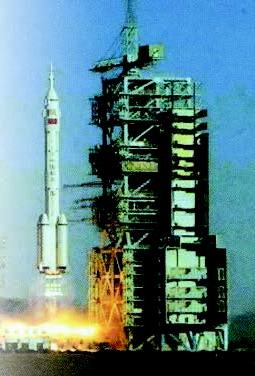
\includegraphics{8-9.pdf}
  \caption{}\label{fig:8-9}
\end{figure}

稀薄气体的辉光放电是怎样形成的呢?

气体稀薄时,气体分子间的距离增大,电子连续两次碰撞所经过的路程加大,因而在电场力作用下获得较大的动能,它们跟中性分子碰撞,会发生电子碰撞电离。
同样的道理,正离子也可以获得较大的动能,跟阴极碰撞时,会从阴极表面打出电子。
于是,气体发生了自激放电。气体的压强越低,发生自激放电需要的电压也越低。

\subsection{弧光放电} 
把两个碳棒分别跟电源的两极相连,让它们接触后再稍稍分离,在两碳棒间就会出现明亮的放电现象,这就是弧光放电。
在大气中产生弧光放电时,两碳棒间的电压并不高,通常只有几十伏,而电流可达几安甚至几十安。
这说明这时气体有很好的导电性,电阻很小。

弧光放电是怎样形成的呢?当两个碳棒相接触时,由于接触处的电阻很大,电流通过时要放出大量的热量,从而使这里的温度升得很高。
当两个碳棒分离后,这样高的温度足以使得气体发生电离和阴极发射电子,于是开始放电。
这就是说,开始产生弧光放电的原因是由于气体和阴极有很高的温度。
使弧光放电维持下来的原因也是由于高温。
被电场加速了的电子和离子跟气体的中性分子碰撞,加剧了气体分子的热运动,使气体温度升得很高,继续发生电离。
被电场加速了的正离子轰击阴极,使阴极保持很高的温度,继续发射电子。
在大气压下的弧光放电,气体的温度高达 \qty{2000}{K} 以上。

弧光放电不仅可以在两个碳棒电极之间发生,也可以在两个金属电极之间发生。

在辉光放电中,如果减少外电路的电阻,使放电电流增大,那么,当电流很强的时候,可以使气体和阴极的温度升得很高,因而辉光放电变成弧光放电。

弧光放电在实际中有着广泛的应用。
弧光放电时发出强光,可以用来制造各种气体放电光源。
弧光放电时放出大量的热量,可以被用来作为热源,如用于电炉炼钢(\cref{fig:8-10})和电焊(\cref{fig:8-11})。
\begin{figure}
  \begin{minipage}[b]{0.48\linewidth}\centering
    \includegraphics{8-10.pdf}
    \caption{电炉炼钢}\label{fig:8-10}
  \end{minipage}
  \begin{minipage}[b]{0.48\linewidth}\centering
    \includegraphics{8-11.pdf}
    \caption{电焊}\label{fig:8-11}
  \end{minipage}
\end{figure}

\subsection{火花放电}
把起电机两电极的放电球互相靠近到几厘米,让起电机起电,随着放电球上电荷的增加,两极间的电势差和电场强度都要增大。
当电场强度增大到一定程度时(约为 \qty{3e6}{V/m}),在两极间就出现一束明亮的、曲折而又分叉的细丝。
这些明亮的细丝很快地穿过两极间的气体,一个接着一个地出现,并且伴有爆炸声。
这就是火花放电。

产生火花放电的电势差的大小跟气体的性质和压强、电极的大小和形状以及两极间的距离等因素有关系。
气体的压强越低,两电极间的距离越小,产生火花放电的电势差就越小。
尖端状电极容易发生放电。
例如在大气压强下,电势差为 \qty{2e4}{V},直径为 \qty{5}{cm} 的球状电极相距 \qty{5.8}{mm} 时产生火花放电,而尖端状电极相距 \qty{15.5}{mm} 即可产生火花放电。

当电源的功率不是很大时,火花放电的放电过程是间断发生的。
这是因为放电时气体被火花击穿,电阻变小,这样在电路里就会有很大的电流,因而引起电势差的重新分布,结果两极间的电势差降到很小,于是停止放电。
接着,当两极间的电势差回升到原来的数值时,又重新开始放电。
当电源的功率足够大时,放电过程可以连续地维持下去,这时火花放电变成弧光放电。

火花放电中使气体电离的原因,是强电场作用下的电子碰撞。
此外,火花本身的辐射也会使气体电离。

闪电是自然界发生的火花放电。
带有相反电荷的两块云,当它们带的电量足够多时,在它们之间就会形成强大的电场,于是发生火花放电。
云层跟大地之间也能够发生闪电,这就是雷击。
根据计算,发生闪电时云层之间或云层和大地之间的电势差可高达几十亿伏,电流强度可达几十万安,而放电时间很短,只有百万分之一秒到百分之一秒。
火花放电路径里的温度很高,常常可以达到 \qty{10000}{K}。
一次闪电放出的能量很大,可达 \qty{e14}{J}。
因此,雷击是一种非常危险的现象,会给人们带来危害。
为了防止雷击,雷雨天不要在高大的树下避雨,电视机、收音机装有室外天线时,要有妥善的接地装置。
高大的建筑物安装避雷针,也是为了避免雷击。

\subsection{电晕放电}
在大气中,当导体的电压很高时,靠近它的地方有很强的电场,能够使空气电离而产生放电。
这种放电只发生在靠近导体的薄的一层空气里,在暗处会看到发出微弱的光,这种放电现象叫做电晕放电。

带电导体的尖端附近电场最强,因而最容易放电。
这种尖端放电就是电晕放电。
如果起电机的放电球上带有尖端,在暗处起电时,就会看到尖端处出现淡紫色光点。
一些高压设备的电极常做成光滑的球面,就是为了避免尖端放电。
高压输电线也会发生电晕放电,这是一种电能损失。
因此高压输电线的表面要做得很光滑,不能有凸起或尖端。

尖端放电也可以被人们所利用,前面提到的避雷针就是一个典型的例子。
避雷针是一个金属的尖端导体,把它安装在建筑物顶端,并用粗铜缆把它与大地接通。
铜缆要接到埋在地下的金属板上,以保持避雷针与大地接触良好。
当带电的云层与建筑物接近时,放电通过避雷针和接地导体这条通路不断进行,避免电荷积累而发生雷击。

\section{气体电光源}
气体放电时能发光,这可以用来制成气体电光源。
气体电光源的种类很多,这里介绍常见的几种。

\subsection{霓虹灯}
霓虹灯是一种稀薄气体放电灯。
把细长的玻璃管弯成所需要的形状,两端装上电极。
玻璃管抽成真空后充入压强几百帕斯卡的稀薄气体,通电时,管里的气体发生辉光放电,发出均匀柔和的光。
把不需要发光的部位的管壁涂黑,就可以显出字形或图案。
霓虹灯需要的电压较高,灯管越细、越长,需要的电压越高。
现在,霓虹灯大都按一定的规格制作,起动时需要的电压约为 \qty{15000}{V},维持正常工作的电压约为 \qty{7500}{V}。
但通过的电流很小,通常不超过 \qty{25}{\micro A}。
管里充入的气体不同,霓虹灯的颜色也不一样。
例如,氖气发橘红色光,氦气发金色光,氩气发淡蓝色光等。
如果在管的内壁涂不同的荧光粉,还可以产生更多的颜色。

霓虹灯的色彩鲜艳夺目,能引人注意,因此在商店、车站、码头等场所常常用它来作招牌、广告和装饰用的灯。
在机场还可以用它来作信号灯。

\subsection{日光灯}
日光灯管的结构如\cref{fig:8-12} 所示。
管的两端各有一条灯丝,管里抽成真空后装入少量的水银,并充有压强约为 \qty{400}{Pa} 的氩气,管的内壁涂有荧光粉。
通电后,水银变成蒸气,发生气体放电。
水银蒸气放电发出的光只有小部分是可见光,大部分是看不见的紫外线。
紫外线射到荧光粉上,使荧光粉发出可见光。
选用适当的荧光粉,可以使灯管发出的光的颜色接近日光,日光灯的名字就是由此而来的。
\begin{figure}
  \includegraphics{8-12.pdf}
  \caption{}\label{fig:8-12}
\end{figure}

日光灯发出的光比较柔和,并且发光效率高,比白炽灯高 \numrange{4}{5} 倍,因此,日光灯广泛地用作室内照明。
但是,日光灯的体积大,还需要镇流器等辅助器件,而且功率也不能做得太大,这使它的应用受到了一定的限制。

\subsection{高压水银灯}
照明用的高压水银灯如\cref{fig:8-13} 所示。
外壳呈椭圆体形,是硬玻璃制成的,起保温作用,防止周围环境对灯的影响。
外壳的内壁涂荧光粉。
中央是耐高温的石英玻璃管,内充一定量的水银和少量氩气,两端装有主电极,其中一个主电极附近有一个辅助电极。
辅助电极跟相邻的主电极之间的距离很近,通常只有 \qtyrange{2}{3}{mm},因此,给灯通电后,这两个电极之间的气体首先发生电离,形成辉光放电。
放电时产生大量的电子和离子,于是引起两主电极的辉光放电,并逐步形成弧光放电。
放电时放出的热量使水银大量蒸发,当水银全部蒸发后,灯管达到稳定工作状态。
从启动到稳定工作状态通常需要 \qtyrange{4}{10}{min}。
气体放电时发出可见光和紫外线,紫外线又使外壳内壁的荧光粉发出可见光,从而得到很强的可见光。
这种灯工作时的温度很高,电弧轴心的温度可达 \qty{5500}{K} 左右,管壁的温度也有 \qtyrange{600}{700}{K}。
在这样高的温度下,管内水银蒸气的压强也很高,约为 \qtyrange{2e5}{6e5}{Pa},高压水银灯的名字就是由此而来的。
相比之下,日光灯的工作温度约为 \qty{300}{K} 多些,这时水银蒸气压只有 \qty{0.8}{Pa}。
因此,日光灯又叫做低压水银灯。

\medskip\noindent
\begin{minipage}{0.7\linewidth}\parindent2em
高压水银灯的体积小、亮度大,因而通常用在街道、广场、仓库等地的照明。
高压水银灯也有它的不足之处。
如上面提到的,启动时间较长,需要 \qtyrange{4}{10}{min},同时不能连续启动,熄灭后要停 \qtyrange{5}{10}{min},等灯的温度下降,管内的压强降低后,才能重新启动。
跟日光灯一样,也需要有镇流器等辅助器件。

除了以上几种气体电光源外,还有超高压水银灯、钠灯和氙灯等。
超高压水银灯的水银蒸气的压强在 \qty{e6}{Pa}以上,亮度比高压水银灯更大。
高压钠灯的发光效率最高,它发出的光呈金黄色,现在大中城市的主要街道上已用它来照明。
氙灯的亮度最大,功率可达几万瓦,常用在大的车站、码头、机场和建筑工地等需要大面积照明的地方。
\end{minipage}\hfill
\begin{minipage}{0.27\linewidth}\centering
\begin{figurehere}
  \includegraphics{8-13.pdf}
  \caption{}\label{fig:8-13}
\end{figurehere}
\end{minipage}\par\medskip

\section{真空中的电流}
在稀薄气体辉光放电的实验中,如果继续抽出管内的空气,当管内的压强降到约 \qty{0.1}{Pa} 的时候,也就是通常所说的抽到真空的时候,就不再发生辉光放电。
这是因为管内的空气相当稀薄,电子在管中运动几乎碰不到气体分子,所以不能使气体电离发光。
这时对着阴极的玻璃管壁却发出荧光;如果在管中放一个十字形的金属片,荧光就出现十字形阴影。
这表明玻璃壁发出的荧光是从阴极发出的一种射线引起的,这种射线叫做\Concept{阴极射线}。产生阴极射线的管子叫做阴极射线管。

为了查明阴极射线的性质,人们做了大量的实验。
在阴极射线管内装一个可以在支架上滚动的叶轮,阴极射线射到叶轮上会使叶轮滚向阳极。
这表明阴极射线是高速运动的粒子流,有很大的动能。

在阴极射线管内装一个涂有荧光物质的板,用来显示阴极射线的轨迹;在阴极射线通路的两侧各装一个极板,把它们接到直流电源的两极上,会看到阴极射线向正极板偏转。
这表明阴极射线是带负电的粒子流。

1897年,英国科学家汤姆生测定了这种粒子的电荷跟质量的比,发现它是带有最小负电荷的粒子,也就是电子。
阴极射线是从阴极发出的电子流。
因此,阴极射线又叫做电子射线,阴极射线管又叫做电子射线管。

前面已说明,这里讲的电子射线管内的压强约为 \qty{0.1}{Pa}。
这种情况下,电子射线的产生,是属于前面讲的正离子轰击发射。
也就是说,正离子在电场的作用下获得很大的动能,它跟阴极碰撞,使阴极发射电子。

\section{示波管}
示波管是一种电子射线管,它的构造如\cref{fig:8-14} 所示。
玻璃管内的真空度很高,可达 \qty{e-4}{Pa}。
在这样高度真空下,它是采用热电子发射的方式来产生电子射线的。
\begin{figure}
  \includegraphics{8-14.pdf}
  \caption{}\label{fig:8-14}
\end{figure}

灯丝通电后温度升高,给阴极加热,使阴极发射电子。
电子经过圆筒形的控制极和阳极的小孔,形成一束很细的加速的电子束。
用来产生电子束的这一部分装置通常叫做电子枪。
从电子枪射出的电子束,打在管底的荧光屏上,形成一个小的亮斑。
亮斑的大小和亮度,由加在控制极和阳极上的电压来控制。

在电子枪的前面是两组偏转极板:水平偏转极板 $XX'$ 和竖直偏转极板 $YY'$。
如果仅在水平偏转极板上加一个电压,例如极板 $X$ 的电势高,极板 $X'$ 的电势低,那么电子束从两极板间通过时就要向极板 $X$ 一边偏转,荧光屏上的亮斑也要向极板 $X$ 方向水平偏移(\cref{fig:8-15a})。
反之,如果极板 $X$ 的电势低,极板 $X'$ 的电势高,亮斑就向极板 $X'$ 方向水平偏移(\cref{fig:8-15b})。
$XX'$ 间的电势差越大,亮斑偏移得越大。
采用特定的电子线路,可以使 $XX'$ 间的电势差从某一负值均匀地上升到某一值,然后迅速地返回原来的负值,再均匀上升,这时荧光屏上的亮斑就从一边匀速地水平移向另一边,然后迅速地返回原处,再匀速地水平移向另一边。
这个过程叫做扫描,加在水平偏转极板上能够产生扫描的电压叫做扫描电压。
当扫描的频率加快时,由于视觉暂留和荧光物质的残光特性,在荧光屏上移动的亮斑看起来成了一条亮线(\cref{fig:8-16})。
\begin{figure}
  \begin{minipage}[b]{0.6\linewidth}\centering
    \begin{minipage}{0.5\linewidth}\raggedleft
      \includegraphics{8-15a.pdf}
      \subcaption{}\label{fig:8-15a}
    \end{minipage}%
    \begin{minipage}{0.5\linewidth}\raggedright
      \includegraphics{8-15b.pdf}
      \subcaption{}\label{fig:8-15b}
    \end{minipage}
    \caption{}\label{fig:8-15}
  \end{minipage}
  \begin{minipage}[b]{0.38\linewidth}\centering
    \includegraphics{8-16.pdf}
    \caption{}\label{fig:8-16}
  \end{minipage}
\end{figure}

同样的道理,给竖直偏转极板 $YY'$ 加一个电压时,荧光屏上的亮斑就要发生竖直偏移,如果 $YY'$ 上的电压随时间变化,那么亮斑将在竖直方向移动,移动的规律跟电压变化的规律相同。

如果在竖直偏转极板上加一个变化的电压,同时又在水平极板上加一个一定频率的扫描电压,那么荧光屏的亮斑在竖直方向移动的同时,又在水平方向匀速移动。
于是,从亮斑的位置变化就可以知道竖直极板上的电压随时间变化的情况。

\medskip\noindent
\begin{minipage}{0.7\linewidth}\parindent2em
通常,加在竖直极板上的要研究的电压是周期性变化的。
如果扫描电压的周期与竖直极板上电压的周期相同,并且起始时间也相同(这在技术上叫做同步),那么,在荧光屏上就可以看到一条稳定的图线。
这时得到的图线表示出竖直极板上的电压在一个周期内随时间而变化的规律。
例如,加在竖直极板上的电压是随时间按正弦规律变化的,它的变化周期与扫描电压的周期相同,起始时间也相同,那么在荧光屏上就显示出一条正弦曲线(\cref{fig:8-17})。
\end{minipage}\hfill
\begin{minipage}{0.25\linewidth}\centering
\begin{figurehere}
  \includegraphics{8-17.pdf}
  \caption{}\label{fig:8-17}
\end{figurehere}
\end{minipage}

\medskip
示波管是示波器的核心部件。
示波器内部的电子线路比较复杂,我们不作具体的研究。
我们将在学生实验里初步学习它的使用方法。
由于电子的惯性很小,电子流的偏转能几乎立即跟上电压的变化,因此,亮斑在荧光屏上的运动能准确地反映偏转极板上电压的微小的或速的变化。
这对于研究各种信号电压的变化情况是很方便的。
此外,如振动、光、温度等的变化,也可以转化成电压的变化,然后用示波器来研究。
示波器已经成了科学研究、检测和修理各种电子仪器不可缺少的工具。


\begin{Practice}
\begin{question}
  \item 放电管里气体的自激放电是怎样形成的?
  \item 为什么安装了避雷针能够避免雷击?
  \item 示波管荧光屏上显示出的一条完整的正弦曲线(\cref{fig:8-17}),是在什么条件下得到的?这时,如果使扫描电压的周期增大为原来的二倍,那么,荧光屏上将显示出什么样的图线?
\end{question}
\end{Practice}


\section{半导体的导电性}
有一类物质,它的导电能力介于导体和绝缘体之间,称为半导体,如硅、锗、氧化亚铜、砷化镓等都是。
用半导体制成的各种器件有着极其广泛的应用,从日常生活到现代通讯设备、电子计算机、空间技术等都离不开它。
半导体对于科学技术的发展已经产生了十分深远的影响。
半导体所以有如此重要的作用,在于它有着自己特殊的导电性质。
下面我们用半导体硅为例来说明。

硅是四价元素,硅原子最外层有四个价电子。
在硅的单晶体中,硅原子的排列是很有规律的,每个原子都以四个价电子与相邻的四个原子联系着。这样,相邻的两个原子就有一对共有电子,形成共价键。
\cref{fig:8-18} 是硅单晶的共价键结构的平面示意图。处于共价键中的电子是一种束缚电子,不能自由移动。
但是,由于热运动,其中极少数电子有可能获得足够的能量,挣脱束缚成为自由电子。在外电场作用下,这些自由电子就逆着电场方向定向移动形成电流,这是半导体的电子导电。
\begin{figure}
  \begin{minipage}[b]{0.48\linewidth}\centering
    \includegraphics{8-18.pdf}
    \caption{}\label{fig:8-18}
  \end{minipage}
  \begin{minipage}[b]{0.48\linewidth}\centering
    \includegraphics{8-19.pdf}
    \caption{}\label{fig:8-19}
  \end{minipage}
\end{figure}

当共价键中的一个束缚电子挣脱为自由电子时,在原来共价键中就留下一个空位,叫做\Concept{空穴}(\cref{fig:8-19})。
我们知道,原子是电中性的,空穴是失去了带负电的电子而形成的,因而可以把空穴看作是带正电的。
这个空穴很容易由附近共价键中的束缚电子来填补,于是又出现了一个新的空穴。
束缚电子的这种填补运动,从效果上看相当于空穴向着相反方向的运动。
为了跟自由电子的移动相区别,把束缚电子的这种填补运动叫做空穴运动。
我们可以打个比方,比如大礼堂里坐满了人,第一排走了一人,出现一个空位,第二排的人向前坐了第一排的空位,第二排又出现一个新的空位,后排的人陆续向前填补。
这样就出现了人的从后往前的填补运动,从效果上看好象空位向后运动一样。
在外电场作用下,空穴顺着电场方向定向移动形成电流,这叫做半导体的\Concept{空穴导电}。

在纯净的半导体中,自由电子和空穴是成对出现的,叫做电子—空穴对。
自由电子和空穴也会重新结合,叫做复合。

可见,半导体导电与金属导电的情况不同。
金属只有电子导电,而半导体既有电子导电又有空穴导电。
金属虽然只有电子导电,但它的自由电子数量很多,导电性好;纯净的半导体虽然有电子导电和空穴导电,但它的自由电子和空穴的数量很少,导电性差。

然而,在某些情况下,半导体也可以产生较多的自由电子和空穴,从而使它的导电性发生明显的改善。
例如,半导体的温度升高或受到光照时,就会使共价键中更多的电子挣脱束缚,形成更多的电子-空穴对,大大增强了它的导电性,这就是半导体的热敏特性和光敏特性,利用半导体的热敏特性和光敏特性可以制成热敏电阻(它的阻值随着温度的高低而明显地变化)和光敏电阻(它的阻值随着光照的强弱而明显地变化)。
热敏电阻和光敏电阻在测温和自动控制中有着重要的应用。

\section{N 型半导体和 P 型半导体}
在纯净的半导体中掺入微量的杂质,会使它的导电性大大增强。
掺入的杂质有两类,因而形成两类半导体。

一类是在纯净的半导体中掺入比它的价电子多的杂质。
例如在硅中掺入微量的五价元素磷 \ce{P}(或砷 \ce{As}、锑 \ce{Sb}),一些硅原子就会被磷原子代替。
磷原子有五个价电子,它与周围硅原子组成共价键时多出一个价电子。
这个价电子受磷原子的束缚很弱,很容易成为自由电子(\cref{fig:8-20})。
磷原子失去一个价电子后成为正离子。
在这类半导体中,每个五价原子都能提供一个自由电子,因而自由电子的数目显著增多。
当然,由于热运动也会产生电子—空穴对,这类半导体中也有少数的空穴,但自由电子的浓度要比空穴的浓度大得多。
这类半导体主要靠电子导电,叫做电子型半导体或\Concept{N 型半导体}。
\begin{figure}
  \begin{minipage}[b]{0.48\linewidth}\centering
    \includegraphics{8-20.pdf}
    \caption{}\label{fig:8-20}
  \end{minipage}
  \begin{minipage}[b]{0.48\linewidth}\centering
    \includegraphics{8-21.pdf}
    \caption{}\label{fig:8-21}
  \end{minipage}
\end{figure}

另一类是在纯净的半导体中掺入比它的价电子少的杂质。
例如在硅中掺入微量的三价元素铟 \ce{In}(或铝 \ce{Al}、镓 \ce{Ga}、硼 \ce{B}),一些硅原子就会被铟原子代替。
铟原子只有三个价电子,它与周围硅原子组成共价键时缺少一个电子,附近共价键中的电子很容易前来填补,从而形成一个空穴(\cref{fig:8-21})。
铟原子得到一个电子后成为负离子。
在这类半导体中,每个三价原子都能提供一个空穴,因而空穴的数目显著增多。
当然,由于热运动会产生电子—空穴对,这类半导体中也有少数自由电子,但是空穴的浓度要比自由电子的浓度大得多。
这类半导体主要靠空穴导电,叫做空穴型半导体或\Concept{P 型半导体}。

\section{PN 结\texorpdfstring{\quad}{ }晶体二极管}
由上节可知,在纯净的半导体中掺入不同的微量杂质,可以使纯净的半导体成为 N 型半导体或 P 型半导体。
用不同的掺杂工艺,也可以使一块纯净的半导体的一边成为 N 型半导体,另一边成为 P 型半导体,这时在 N 型和 P 型的交界处形成一个具有特殊性质的区域,叫做 PN 结。
正是由于 PN 结的形成,才产生了各种类型的半导体器件;PN 结是组成晶体二极管、晶体三极管及其他半导体器件的基础。
\begin{figure}
  \includegraphics{8-22.pdf}
  \caption{}\label{fig:8-22}
\end{figure}

现在我们讨论 PN 结的形成。
我们知道,N 型半导体中自由电子的浓度大,P 型半导体中空穴的浓度大。
把 N 型和 P 型半导体结合在一起时,在它们的交界面处,自由电子要从 N 区向 P 区扩散并与 P 区的空穴复合,空穴要从 P 区向 N 区扩散并与 N 区的自由电子复合(\cref{fig:8-22})。

扩散之前,N 型和 P 型半导体都是电中性的,在交界面处没有电场。
扩散开始后,在靠近交界面处,N 区一边由于跑掉了自由电子而留下了带正电的离子,P 区一边由于跑掉了空穴而留下了带负电的离子。
这些不能移动的带电离子集中在交界面附近,形成了一个电场,其方向从带正电的 N 区指向带负电的 P 区。
显然,这个电场的作用是阻止自由电子向 P 区和空穴向 N 区进行扩散。
因此,N 型和 P 型半导体交界面处附近的带电离子区叫做阻挡层,它形成的电场叫做阻挡层电场(\cref{fig:8-23})。
随着扩散运动的进行,阻挡层电场增强,扩散运动减弱,最后达到稳定状态,在 N 型和 P 型半导体交界面处形成一个很薄的阻挡层,这就是\Concept{PN 结}。
\begin{figure}
  \begin{minipage}[b]{0.48\linewidth}\centering
    \includegraphics{8-23.pdf}
    \caption{}\label{fig:8-23}
  \end{minipage}
  \begin{minipage}[b]{0.48\linewidth}\centering
    \includegraphics{8-24.pdf}
    \caption{}\label{fig:8-24}
  \end{minipage}
\end{figure}

在 PN 结的 N 区和 P 区各引出一个电极,再装上管壳,就成了一个晶体二极管。
跟 N 区相连的是晶体二极管的负极,跟 P 区相连的是晶体二极管的正极(\cref{fig:8-24})。
晶体二极管按结构可分为点接触型和面接触型两类,如\cref{fig:8-25} 所示。
\begin{figure}
  \begin{minipage}[b]{0.45\linewidth}\centering
    \includegraphics{8-25a.pdf}
    \subcaption{点接触型}\label{fig:8-25a}
  \end{minipage}
  \begin{minipage}[b]{0.45\linewidth}\centering
    \includegraphics{8-25b.pdf}
    \subcaption{面接触型}\label{fig:8-25b}
  \end{minipage}
  \caption{}\label{fig:8-25}
\end{figure}

\begin{figure}
  \begin{minipage}{0.45\linewidth}\centering
    \includegraphics{8-26a.pdf}
    \subcaption{}\label{fig:8-26a}
  \end{minipage}
  \begin{minipage}{0.45\linewidth}\centering
    \includegraphics{8-26b.pdf}
    \subcaption{}\label{fig:8-26b}
  \end{minipage}
  \caption{}\label{fig:8-26}
\end{figure}

把二极管、小灯泡和电池象\cref{fig:8-26a} 那样连成电路,这时小灯泡发光。
可是把电池的正负极互相调换,象\cref{fig:8-26b} 那样连成电路,小灯泡就不发光了。
可见晶体二极管只允许一个方向的电流通过,也就是说,晶体二极管有单向导电性。

现在我们简单地说明一下晶体二极管单向导电性的原因。
象\cref{fig:8-27a} 那样,当 N 区接电源的负极,P 区接电源的正极时,电源加在晶体管上的外电场方向跟阻挡层的电场方向相反,削弱了阻挡层电场,阻挡层变薄。
这时 N 区的自由电子和 P 区的空穴可以顺利地通过 PN 结,在外电场的作用下形成电流,使小灯泡发光。
象\cref{fig:8-27b} 那样,当 N 区接电源的正极,P 区接电源的负极时,加在晶体管上的外电场方向跟阻挡层的电场方向相同,增强了阻挡层电场,阻挡层变厚。
这时 P 区的自由电子和 N 区的空穴可以通过 PN 结,在外电场的作用下形成反向电流。
但是,P 区的自由电子和 N 区的空穴都很少,所以反向电流很小,粗略地可以认为没有电流通过,不能使小灯泡发光。因此晶体二极管表现为单向导电。
\begin{figure}
  \begin{minipage}[b]{0.48\linewidth}\centering
    \includegraphics{8-27a.pdf}
    \subcaption{}\label{fig:8-27a}
  \end{minipage}
  \begin{minipage}[b]{0.48\linewidth}\centering
    \includegraphics{8-27b.pdf}
    \subcaption{}\label{fig:8-27b}
  \end{minipage}
  \caption{}\label{fig:8-27}
\end{figure}

\section{晶体三极管}
\subsection{晶体三极管的结构}
晶体三极管由两个 PN 结、三个电极线和管壳构成,分为 PNP 型和 NPN 型两类。\cref{fig:8-28} 是 PNP 型的结构和符号,\cref{fig:8-29} 是 NPN 型的结构和符号。
\begin{figure}
  \includegraphics{8-28.pdf}
  \caption{PNP 型晶体三极管}\label{fig:8-28}
\end{figure}

\begin{figure}
  \includegraphics{8-29.pdf}
  \caption{NPN 型晶体三极管}\label{fig:8-29}
\end{figure}

从图可以看出,晶体三极管内分三个区:\Concept{发射区、基区、集电区}。
它们各有一条电极引线,分别叫\Concept{发射极 $e$}、\Concept{基极 $b$} 和\Concept{集电极 $c$}。
符号图中的发射极的箭头方向表示电流方向。发射区与基区之间的 PN 结叫做\Concept{发射结},集电区与基区之间的 PN 结叫做\Concept{集电结}。

发射区和集电区是同一类型的半导体,但它们并不完全相同。
发射区的杂质浓度较大,跟基区的接触面积较小。
集电区的杂质浓度较小,跟基区的接触面积较大。
基区很薄,杂质浓度更小。
由于在结构上有这些特点,晶体三极管(以下简称三极管)并不等于两个二极管的简单组合,而有许多新的性能,最重要的是具有放大作用。

\subsection{三极管的放大作用}

PNP 型和 NPN 型三极管的工作原理是相同的,我们以 PNP 型为例来研究三极管的放大作用。

把一个 PNP 型三极管按照\cref{fig:8-30} 那样连接在电路中,从串联在电路中的毫安表和微安表可以读出通过发射极的电流 $I_e$、通过基极的电流 $I_b$ 和通过集电极的电流$I_c$。
电路中的 $R$ 是限流电阻,$W$ 是电位器。
当改变电位器 $W$ 的阻值时,基极电流 $I_b$ 就改变,同时集电极电流 $I_c$ 和发射极电流 $I_e$ 也随着改变。
为了研究 $I_b$、$I_c$、$I_e$ 之间的关系,我们可以多次改变 $W$ 的阻值,把每次的 $I_b$、$I_c$ 和 $I_e$ 的值都记录下来,\cref{tab:8-2} 是某个三极管的测试记录。
\begin{figure}
  \begin{minipage}[b]{0.48\linewidth}\centering
    \includegraphics{8-30.pdf}
    \caption{}\label{fig:8-30}
  \end{minipage}
  \begin{minipage}[b]{0.48\linewidth}\centering
    \includegraphics{8-31.pdf}
    \caption{}\label{fig:8-31}
  \end{minipage}
\end{figure}

\begin{table}
  \caption{某个三极管的测试记录}\label{tab:8-2}
  \begin{tblr}{colspec={c*{10}{X[r]}},hline{2}=0.8pt,row{1}={m,c}}
测量次数  & 1&2&3&4&5&6&7&8&9&10\\
$I_b$(\unit{mA})& 0.00 & 0.01 & 0.02 & 0.03 & 0.04 & 0.05 &0.10  & 0.20 & 0.30 & 0.50 \\ 
$I_c$(\unit{mA})& 0.10 & 0.50 & 0.95 & 1.42 & 1.91 & 2.41 & 4.91 & 9.51 & 13.7 & 21.3 \\
$I_e$(\unit{mA})& 0.10 & 0.51 & 0.97 & 1.45 & 1.96 & 2.46 & 5.01 & 9.71 & 14.0 & 21.8 \\  
  \end{tblr}
\end{table}

从测试记录可以看出,发射极电流总是等于基极电流和集电极电流之和:$I_e=I_b+I_c$,而且基极电流远小于集电极电流:$I_b\ll I_c$。
这说明发射极电流流进三极管后分成两部分,小部分由基极流出,大部分由集电极流出。
三极管的这种电流分配关系可用\cref{fig:8-31} 形象地表示出来。

从测试记录还可以看出,当基极电流稍有变化时,集电极电流就有较大的变化。
例如,当基极电流 $I_b$ 从 \qty{0.01}{mA} 变到 \qty{0.02}{mA} 时,集电极电流就由 \qty{0.50}{mA} 变到 \qty{0.95}{mA}。
基极电流的变化量 $\Delta I_b$ 只有 \qty{0.01}{mA},而集电极电流的变化量 $\Delta I_c$ 却有 \qty{0.45}{mA}。
集电极电流的变化量是基极电流变化量的 45 倍,三极管的这种作用叫做它的放大作用。

由于三极管有放大作用,因此获得了广泛地应用。
三极管的放大作用也可以根据 PN 结的性质作出解释,本书就不讲了。

\begin{Review}
\begin{question}
  \item 金属中的电流是怎样形成的?简述用电子论的观点解释欧姆定律。
  \item 电解质中的电流是怎样形成的?电解质导电跟金属导电有什么不同?
  \item 法拉第电解第一定律的内容是什么?法拉第电解第二定律的内容是什么?法拉第恒量的意义是什么?法拉第恒量、基本电荷、阿伏伽德罗常数三者之间的关系是怎样的?
  \item 气体导电跟金属导电和电解质导电有什么相同点和不同点?
  \item 什么是气体放电?什么是被激放电和自激放电?简述自激放电的几种形式。
  \item 为什么说阴极射线是从阴极发出的电子流?
  \item 简述示波管的构造和它的工作原理。
  \item 半导体的导电特点是什么?什么是 N 型半导体?什么是 P 型半导体?
  \item 什么是 PN 结?它是怎样形成的?
  \item 为什么晶体二极管有单向导电性?
  \item 什么是晶体三极管的放大作用?
\end{question}
\end{Review}